\begin{figure}[htb]
    \centering
        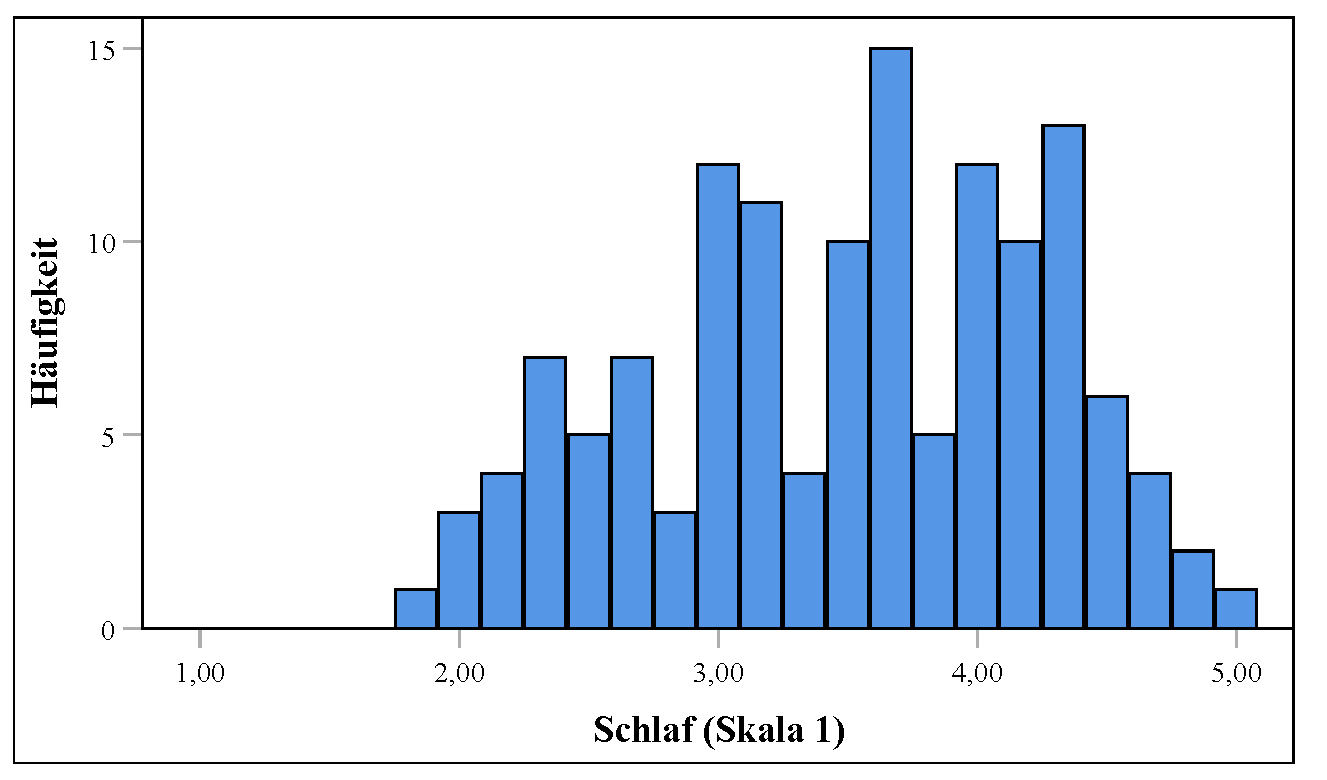
\includegraphics[width=0.8\linewidth]{Histogramm Skala Schlaf.pdf}
        \caption[Histogramm für die Skala Schlaf]{Histogramm für die Skala Schlaf. 
        Codierung: 1.00 = stimme nicht zu ... 5.00~=~stimme vollständig zu. $N = 135$. 
        $M = 3.50$, $SD = 0.76$, $Skewness = -0.25$, $Kurtosis = 0.86$, 
        Cronbachs-\textalpha \ = .72.}
        \label{Histogramm Skala Schlaf}
\end{figure}